% 
% Annual Cognitive Science Conference
% Sample LaTeX Paper -- Proceedings Format
% 

% Original : Ashwin Ram (ashwin@cc.gatech.edu)       04/01/1994
% Modified : Johanna Moore (jmoore@cs.pitt.edu)      03/17/1995
% Modified : David Noelle (noelle@ucsd.edu)          03/15/1996
% Modified : Pat Langley (langley@cs.stanford.edu)   01/26/1997
% Latex2e corrections by Ramin Charles Nakisa        01/28/1997 
% Modified : Tina Eliassi-Rad (eliassi@cs.wisc.edu)  01/31/1998
% Modified : Trisha Yannuzzi (trisha@ircs.upenn.edu) 12/28/1999 (in process)
% Modified : Mary Ellen Foster (M.E.Foster@ed.ac.uk) 12/11/2000
% Modified : Ken Forbus                              01/23/2004
% Modified : Eli M. Silk (esilk@pitt.edu)            05/24/2005
% Modified : Niels Taatgen (taatgen@cmu.edu)         10/24/2006
% Modified : David Noelle (dnoelle@ucmerced.edu)     11/19/2014

%% Change "letterpaper" in the following line to "a4paper" if you must.

\documentclass[10pt,letterpaper]{article}

\usepackage{cogsci}
\usepackage{pslatex}
\usepackage{apacite}
\usepackage{graphicx}
\usepackage{float}

\title{Computational Cognitive Modeling, Spring 2021 - Final Project}
 
\author{{\large \bf João Galinho (jg6606@nyu.edu)} \\
  NYU Graduate School of Arts and Science, Department of Computer Science
  \AND {\large \bf Sara Okun (sjo302@nyu.edu)} \\
  NYU Graduate School of Arts and Science, Center for Data Science
  \AND {\large \bf Keshav Pant (kp2749@nyu.edu)} \\
  NYU Graduate School of Arts and Science, Center for Data Science}


\begin{document}

\maketitle


\section{Introduction}
Past research has indicated that rewards sculpt which set of actions are adopted in a given context \cite{Bitterman2006, Pavlov1927, Schreurs2013}. Classical conditioning builds expectations and predictions of outcomes through repeated pairings of the conditioned and unconditioned stimuli to evoke a particular response \cite{Bitterman2006, Pavlov1927}. Dopamine neurons in the brain have been found to illicit specific response patterns during learning. It has been found that these neurons code for prediction error, suggesting that the brain has neural code that supports reinforcement learning algorithms like temporal difference learning \cite{Schultz2016}. 


\subsection{Temporal Difference Reinforcement Learning}
Temporal difference learning is a model-free reinforcement learning algorithm that learns by tracking values associated with particular states at particular times \cite{SimonDaw2012}. The value function that is updated when utilizing this reinforcement learning algorithm is

\begin{equation}
V_t = V_t + \eta(r_{t+1} + V_{t+1} - V_t)
\end{equation}
where $V_t$ is the value of the current state, $r_{t+1}$ is the reward on the subsequent state, $V_{t+1}$ is the value of the subsequent state and $\eta$ is the learning factor/rate (or step size). In this value function, the prediction error is given by $r_{t+1} + V_{t+1} - V_t$ \cite{Pan2005}. Prediction error will be nonzero when there is a difference between what the value is expected to be and what the reward is. A positive prediction error occurs when a reward was not expected (i.e. a state value of 0 and a positive reward value) and a negative prediction error occurs when a reward is expected, but none was received (i.e. a positive state value and a reward of 0).


\subsection{Dopamine Neurons}
Research has shown that there is a similar pattern of processing in individual dopamine neurons in the brains of animals \cite{Diederen2020, Pan2005, Schultz2016}. Early in learning, dopamine neurons respond when a reward is presented. After many trials and a conditioned stimulus is presented, the neuron's response starts shifting back to the trial at which the conditioned stimulus is presented, until eventually the neuron responds to the conditioned stimulus and not to the reward \cite{Pan2005, Schultz2016}. It has also been shown that if the reward is not presented when there was an expectation of a reward, there is a "dip" in the firing rate of the neuron. 

\begin{figure}[H]
   \centering
    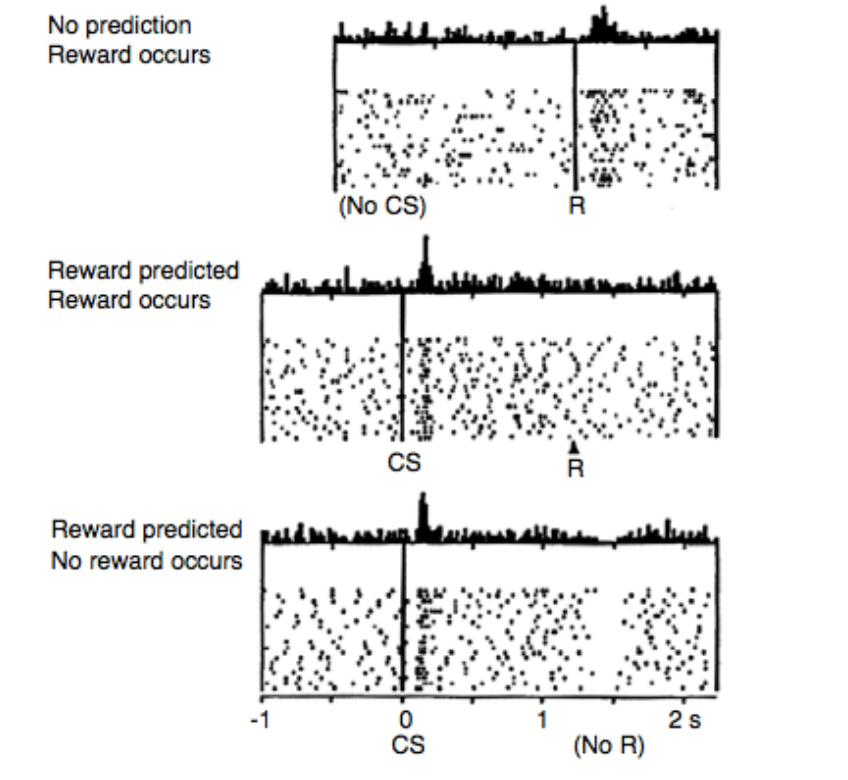
\includegraphics[width = 75mm]{graphs/dopamine.png}
    \caption{Dopamine neurons action potentials \& conditioned stimuli
    \newline \emph{Dopamine neuron electrode recordings from animal brain showing response with just reward, a conditioned stimulus and a reward, and a conditioned stimulus and no reward (both after learning the conditioned stimulus).}}
    \label{fig:Dopamine Neurons}
\end{figure}

This shows that the pattern of response from the dopamine neurons is coding for prediction error and also supports the idea that the temporal difference reinforcement learning algorithm captures some of the basic ingredients of learning processes taking place in the brain \cite{Pan2005,ReddishJohnson2004}.


\subsection{Dopamine and Human Addiction}
Various theories of drug abuse propose that addiction results from behavioral control transitioning from a voluntary system to something more habitual \cite{RobbinsEveritt1999, Tiffany1990}. This is consistent with evidence suggesting that drug abuse and addiction act through mechanisms involving areas of the brain that are involved in dopamine production \cite{RobbinsEveritt1999, WiseBozarth1987}. For instance, studies have shown that when non-addicted healthy adults take stimulants their dopamine response increases, consistent with the expected response activity from dopamine neurons. However, individuals that have a drug addiction show a blunted dopamine release in response to taking stimulants (it is important to note that stimulants are not representative of all drugs, and that different types of drugs have been shown to have different effects on dopamine response) \cite{Nuttetal2015}. 

Although the study of drugs has focused on dopamine response, there are other neurotransmitter systems that are greatly affected by drug use. However, many of those have been shown to influence areas of the brain involving dopamine upon the receipt of drugs \cite{WiseBozarth1987}. As such, for this project we will focus on dopamine neurons and their relation to drug abuse. Some of the areas involved in dopamine production are shown in the figure below.

\begin{figure}[H]
   \centering
    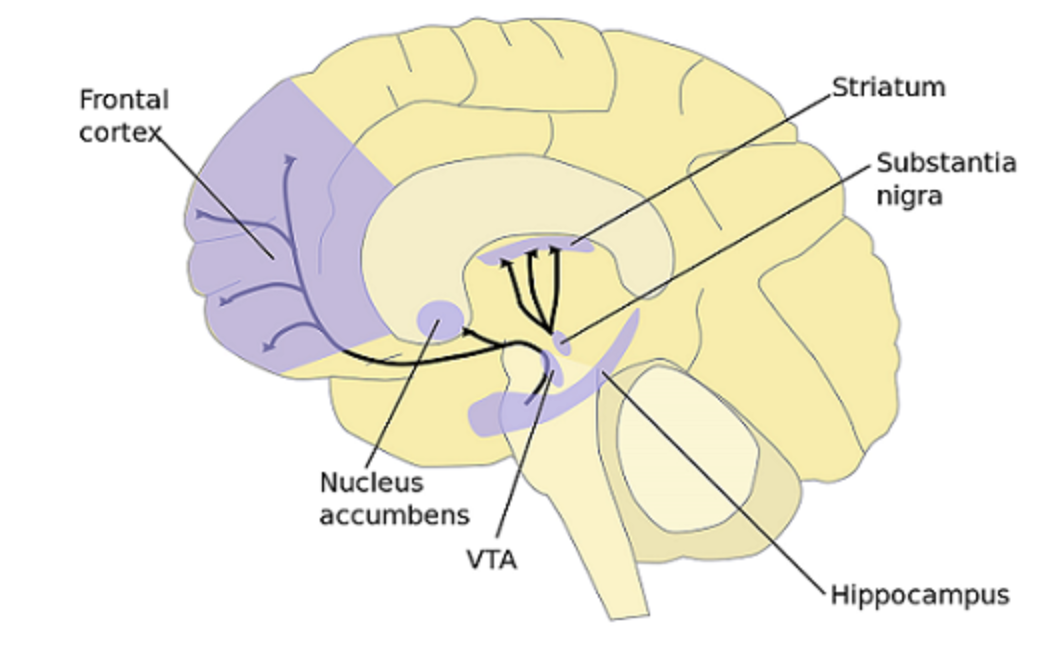
\includegraphics[width = 85mm]{graphs/brain.png}
    \caption{Areas of the brain involved in dopamine production
    \newline \emph{Dopamine neurons are often produced in the VTA. It has therefore been theorized that the VTA is a center for prediction error signals that are propagated to other parts of the cortex that help us update value representations.}}
    \label{fig:Dopamine Brain}
\end{figure}

The behaviors that result from drug abuse have been modeled using model-free reinforcement learning algorithms like temporal difference learning \cite{ReddishJohnson2004, ReddishJensenJohnson2008, SimonDaw2012}. For our project we plan to implement a reinforcement learning model using a temporal difference learning algorithm that inappropriately learns to select an addictive stimulus \cite{ReddishJensenJohnson2008}. We have used the model constructed by Reddish and Johnson (2004) as a basis for our experimentation, which is founded on evidence that a large number of drugs either directly or indirectly cause a spike in dopamine levels \cite{Laviolette2004,Ritz1987, ReddishJohnson2004,ReddishJensenJohnson2008, Piccato1998, Pidoplichko1997}.
We plan to see how different types of agents (agents predisposed to addiction vs healthy controls) learn values and how their prediction errors compare. We will evaluate how well the model and environment we set up relates to findings concerning human addiction from the literature.


\section{Methods}
\subsection{Setting up the environment}
Our model is based off of the Reddish and Johnson (2004) temporal difference model of drug addiction. As previously stated, this algorithm chooses actions to maximize future reward. The algorithm learns state values using equation 1 from the introduction. A discounting factor can be added into the calculation of the prediction error, representing the balance between the importance given to immediate and delayed rewards.

\begin{equation}
\delta(t) = (r_{t+1} + \gamma\, V_{t+1}) - V_t
\end{equation}

$\delta(t)$ represents the prediction error and $\gamma$ is the discounting factor. The value update is then calculated using equation 1, where the prediction error above replaces the previous formulation.

\begin{equation}
V_t = V_t + \eta(\delta(t))
\end{equation}

In temporal difference learning, learning stops when the agent correctly learns the reward. When this occurs, the value of the prediction error is 0, because there is no difference between the expected value $V_t$ and the actual value, given by $r_{t+1} + \gamma\, V_{t+1}$. In terms of dopamine neuron signals, this corresponds to no action potentials being produced.

In our formulation of addiction, we utilized evidence (as in Reddish and Johnson (2004)) that addictive drugs produce an increase in dopamine through neuropharmacological mechanisms \cite{Lowinson2005, Ritz1987}, which can be modeled by producing a positive prediction error regardless of the update of the value function \cite{ReddishJohnson2004, ReddishJensenJohnson2008}. This is achieved by reformulating the definition of prediction error.

\begin{equation}
\delta(t) = \max\left\{(r_{t+1} + \gamma\, V_{t+1}) - V_t + D_t,\ D_t\right\}
\end{equation}

This corresponds to a positive prediction error at every value update when $D_t > 0$. This means that an addicted agent will be subject to a substance in which $D_t > 0$, whereas a non-addicted agent will only be subject to natural rewards with $D_t = 0$. In order to still allow for negative prediction errors, this reduces to the original definition of prediction error in equation 2, without the 'max' operator, whenever $D_t = 0$.


\subsection{Addicted vs. Non-addicted agents}
In this model, an addicted agent is one that is trained with an addictive substance with a value of $D_t > 0$, whereas that dopamine hit related to the addictive substance will not be present in a non-addicted agent trained exclusively with natural rewards that have $D_t=0$. In summary, our definition of addiction involves the introduction of an addictive substance with a reward $r_t$ and also a nonzero dopamine hit $D_t$. Thus, addicted and non-addicted agents will have different baseline patterns when trained in the same environment (Figure 3).

\begin{figure}[H]
   \centering
    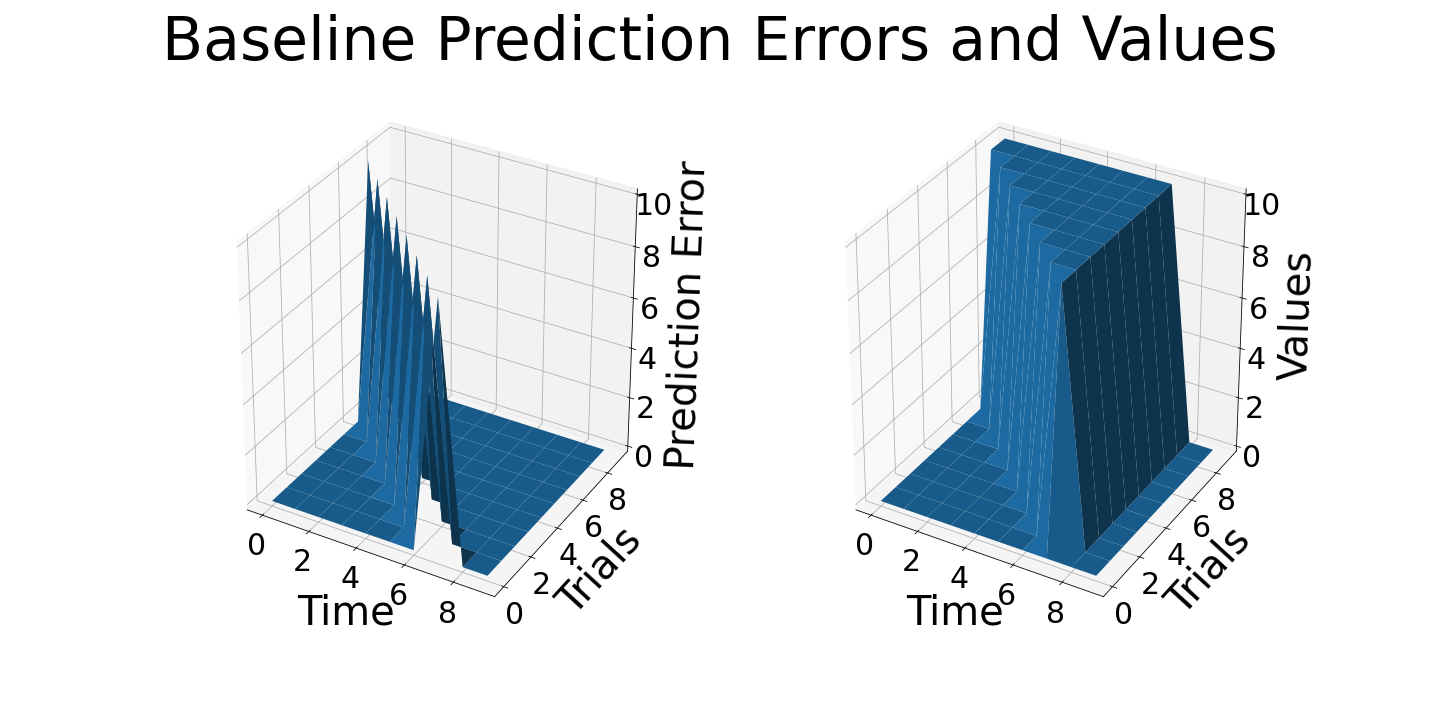
\includegraphics[width = 85mm]{graphs/comp.png}
    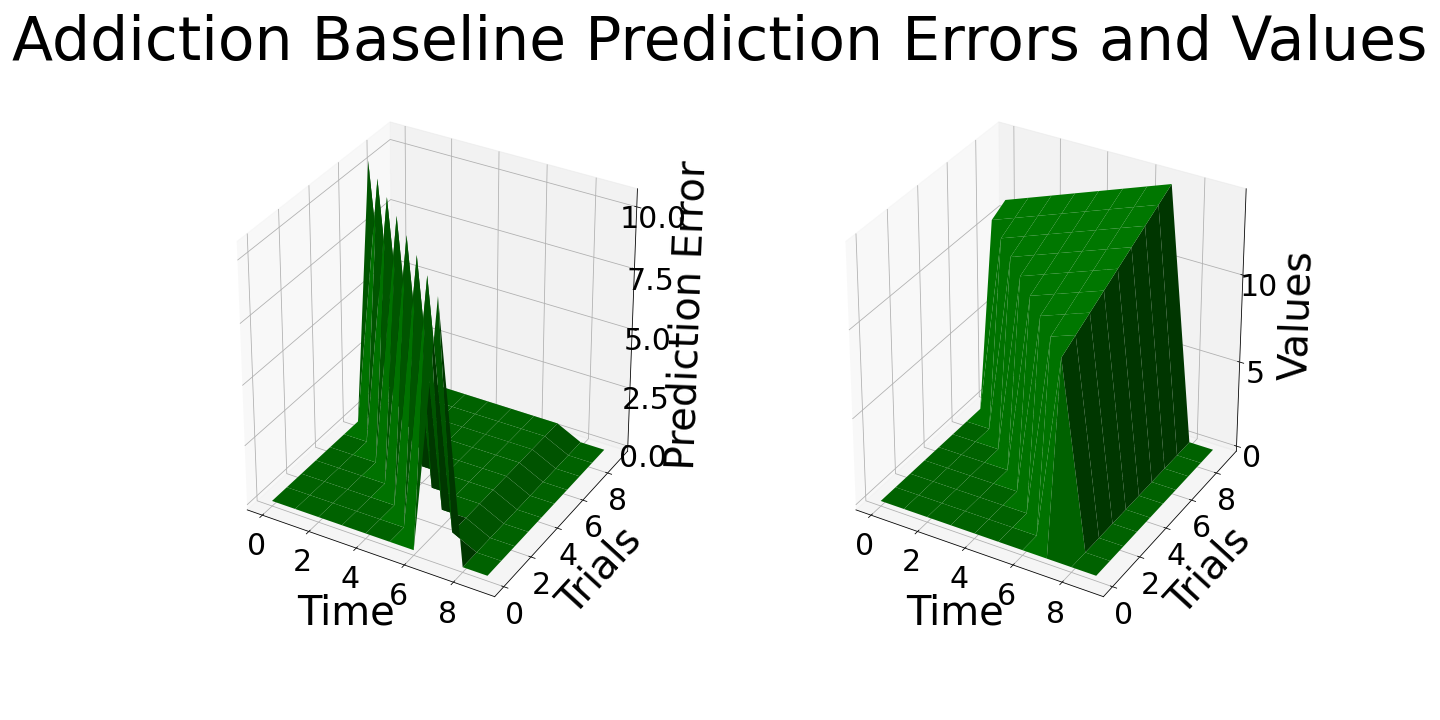
\includegraphics[width = 85mm]{graphs/addicted_comparison.png}
    \caption{Baseline prediction errors and values learned for non-addicted and addicted agents with identical learning parameters (Appendix A: Table 1)
    \newline \emph{Top row: Prediction errors and values for the non-addicted agent. These patterns are consistent with how the TD reinforcement learning algorithm should behave as well as how dopamine neurons respond to rewards. \newline Bottom row: Prediction errors and values for the addicted agent. This illustrates our definition of addiction, as it can be seen that the value for the addictive substance is steadily increasing over time compared to a non-addictive natural reward.}}
    \label{fig:Baseline}
\end{figure}

\vspace{4.5em}

\subsection{Experiment 1: Parameter Testing}
It is important to note that before any experimentation we confirmed that the model we produced is consistent with the patterns of dopamine neuron firing that we discussed in the introduction. For example, we confirmed that when an agent is trained to expect a reward, and then one is not given, a negative prediction error is produced (Figure 4). 

In this experiment we analyze how removing the reward and addiction component of the addictive substance from an addicted agent changed the prediction error and value response patterns. To do this we trained an addicted agent with particular addictive substance parameters, $r_t$ and $D_t$. After a certain number of trials, we removed both the reward and addiction component of the addictive substance (i.e. we set these values to 0 for the remaining trials).

\begin{figure}[H]
   \centering
    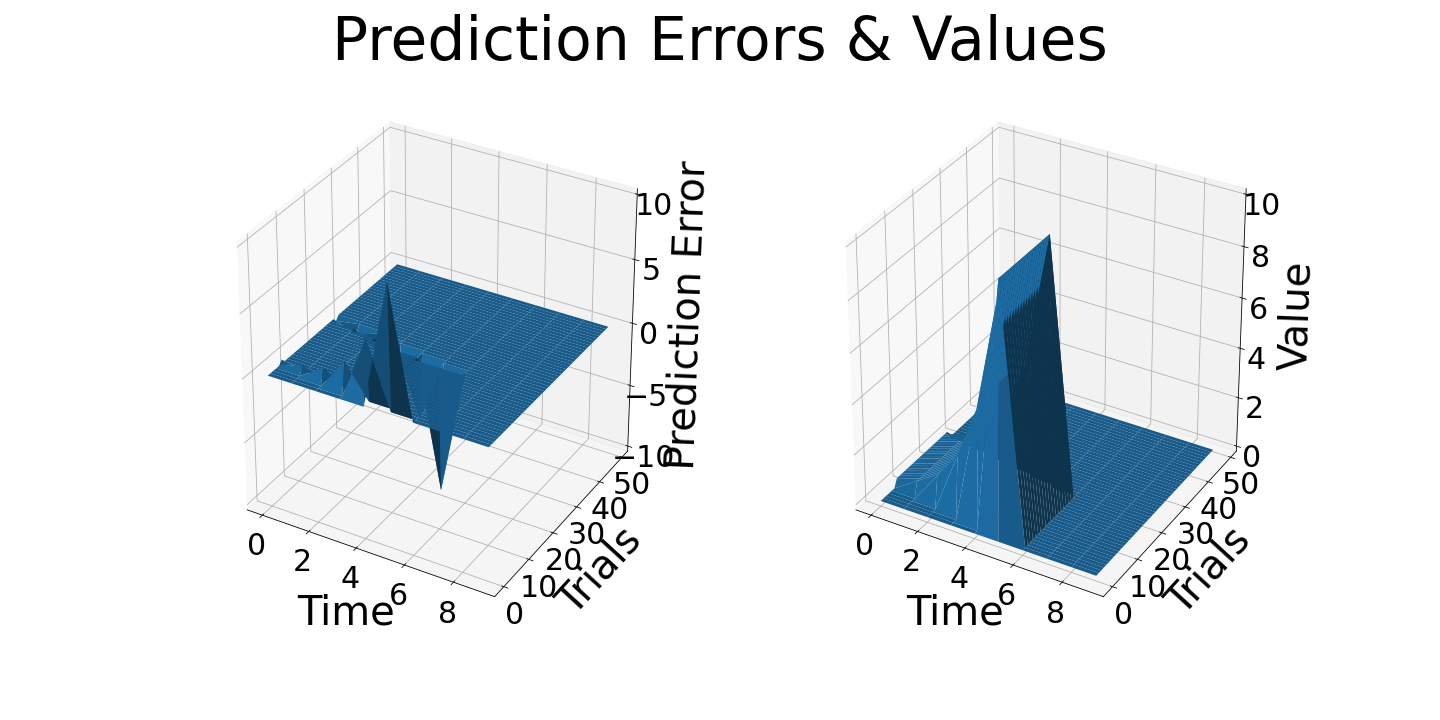
\includegraphics[width = 85mm]{graphs/negPE.png}
    \caption{Negative prediction error when a reward is withdrawn
    \newline \emph{A non-addicted agent is trained for 20 trials to expect a reward at a particular position. When this reward is not given on the remaining trials a negative prediction error occurs, which is consistent with what is seen with dopamine neurons in this scenario.}}
    \label{fig:Baseline}
\end{figure}


\subsection{Experiment 2: Cost}
In this experiment we explore how incrementally decreasing the reward associated with an addictive substance would affect the prediction error and value response patterns. To do this we trained an agent with an addictive substance with a constant reward and addiction component for a certain number of trials. After the agent has learned to expect the reward associated with the addictive substance, we decrease the reward component over the remaining trials. 


\subsection{Experiment 3: Learning/Unlearning}
Our final experiment looks into the time taken to learn and unlearn addicted value structures. One important component to understanding addiction in animals is how long one takes to become addicted to a substance, and also how long it takes to "unlearn" that behavior (i.e. recover). Since experiments of this nature would be extremely unethical to be performed on human subjects, RL models provide a potentially useful alternative. With that in mind, we attempted to map and quantify the time taken for an agent to become addicted and return to normal after the addiction component was removed.

For each specific parameter combination, we first trained a baseline agent with no addiction component, with a large and a small natural reward. We used the converged value table of this agent as a baseline to then compare to the addicted agent's value table. Next, we trained an agent with the same reward structure, with an additional addiction component attached to the small reward time-step. We then defined the "addiction point" as the earliest trial where the agent valued the smaller, addictive reward over the larger, natural one. Finally, we trained a third model, which removed the addiction component for all trials after the previously found addiction point. We defined the "recovery point" as the number of trials before the value table returned to baseline.


\section{Results}
\subsection{Experiment 1: Parameter Testing}
As shown in Figure 5, we know that, in both the model and in how dopamine neurons respond, when a reward is expected and one is not given, a negative prediction error occurs (or a "dip" in the firing rate in the case of biological neurons). Our first experiment tests removing different components of an addictive substance from an agent trained with nonzero addictive substance parameters. Figure 5 shows the result when the addictive substance is not presented to an agent that expects it. The model was trained to expect the addictive substance at time $t = 8$, and the substance was taken away after 10 trials. From the prediction error, it can be seen that this causes a large negative prediction error. The value function also ceases to increase. These results look similar to the response when a non-addictive reward is expected and one is not provided, albeit with a more negative prediction error relative to the reward size.

\begin{figure}[H]
   \centering
    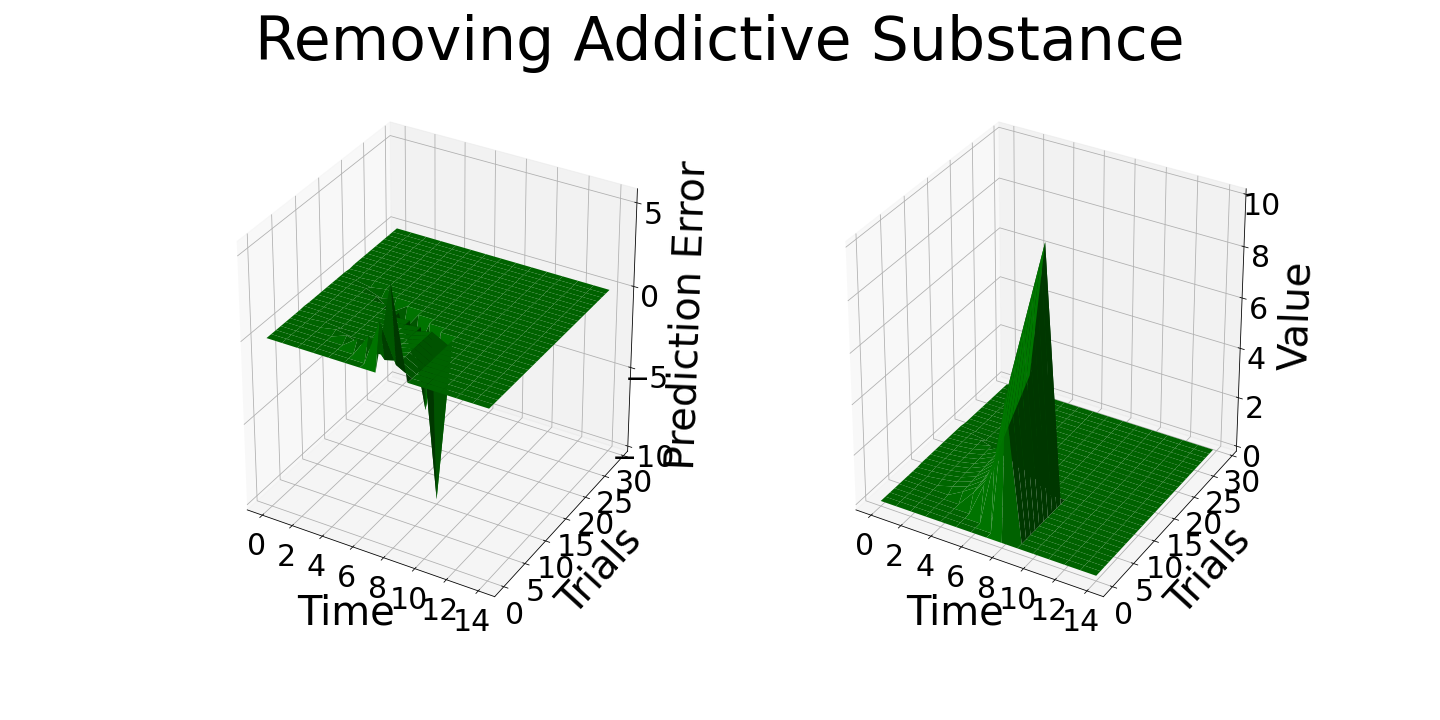
\includegraphics[width = 85mm]{graphs/add_remove.png}
    \caption{Removing an addictive substance from an addicted agent after training
    \newline \emph{An addicted agent is trained for 10 trials to expect an addictive substance at a particular time. The addictive substance is then not supplied for the remaining trials and a negative prediction error occurs, which is similar to what is seen when taking a non-addictive reward away, in both the model and dopamine neurons' response.}}
    \label{fig:Baseline}
\end{figure}

We also experimented with how removing individual components of the addictive substance from the trained addicted agent would change the patterns in prediction error and value. As previously mentioned, the addictive substance has both a reward and an addiction component. Figures 6 and 7 show the results when each are individually removed after training. Removing the reward component of the addictive substance after a certain number of trials causes a decrease in the prediction error, but the value function still continues to grow. Even though the reward portion of the addictive substance has been removed (i.e. the substance no longer has value), the agent is still learning to increasingly value the substance, which is consistent with literature on addiction in humans \cite{Hyman2001, Koob1992}. Removing the addiction component from the addictive substance after a certain number of trials results in a similar prediction error pattern to removing the substance entirely; there is a negative prediction error where the agent expects to receive the addictive substance. The value function also begins to change where the addiction component is removed, starting to converge, as expected, to a value function associated with a non-addictive reward.

\begin{figure}[H]
   \centering
    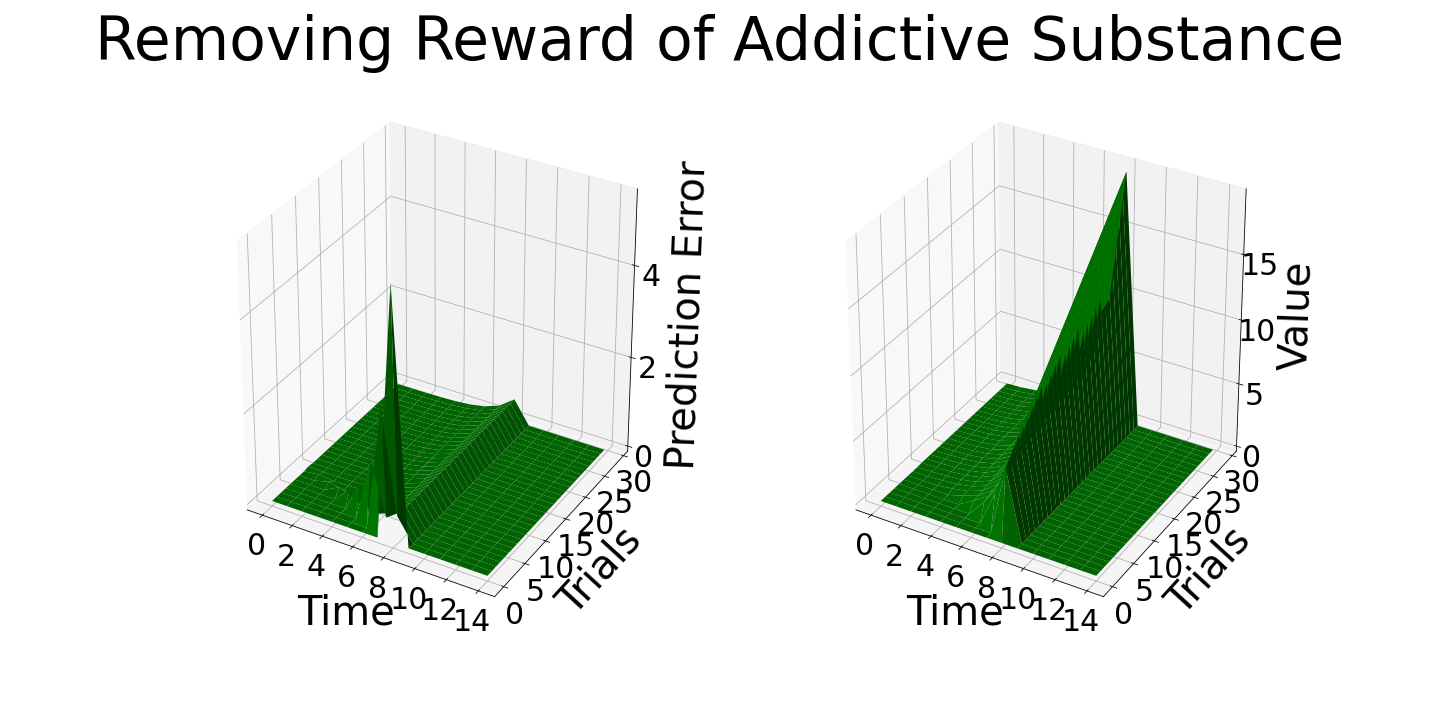
\includegraphics[width = 85mm]{graphs/add_rew_remove.png}
    \caption{Removing the reward component of an addictive substance from an addicted agent after training
    \newline \emph{An addicted agent is trained for 10 trials to expect an addictive substance with particular reward and addiction component at a specific time. The reward component of the addictive substance is then set to 0 for the remaining trials. This results in a decrease in prediction error, but the value function still continues to grow.}}
    \label{fig:Baseline}
\end{figure}

\begin{figure}[H]
   \centering
    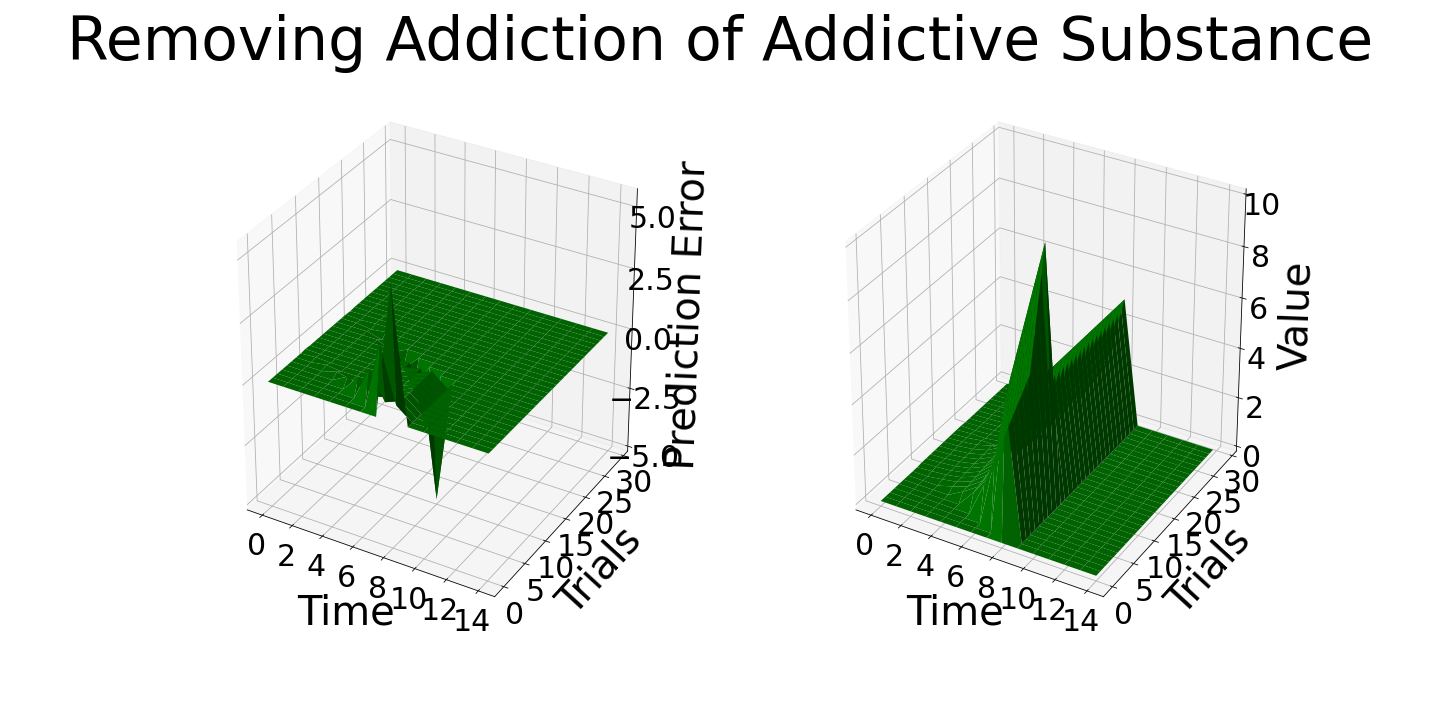
\includegraphics[width = 85mm]{graphs/add_sub_rem.png}
    \caption{Removing the addiction component of an addictive substance from an addicted agent after training
    \newline \emph{An addicted agent is trained for 10 trials to expect an addictive substance with particular reward and addiction component at a specific time. The addiction component of the addictive substance is then set to 0 for the remaining trials. This results in a negative prediction error, and the value function converges to a constant baseline.}}
    \label{fig:Baseline}
\end{figure}


\subsection{Experiment 2: Cost}
The goal of this experiment is to determine how prediction error and the overall value function would change if the reward associated with an addictive substance is decreased after training an addicted agent. The agent was also trained to expect a non-addictive reward in this experiment, so that we could compare the differences between receiving a reward that is constant, and an addictive substance whose reward component decreases over time. This experiment illustrates that, after learning to expect an addictive component with a particular reward value, a decrease in prediction error, up to a certain point, will result from decreasing that reward component. Although the reward component of the addictive substance decreases substantially, the value function associated with the addictive function still increases steadily, as was the case in experiment 1 where the reward component was removed altogether.

\begin{figure}[H]
   \centering
    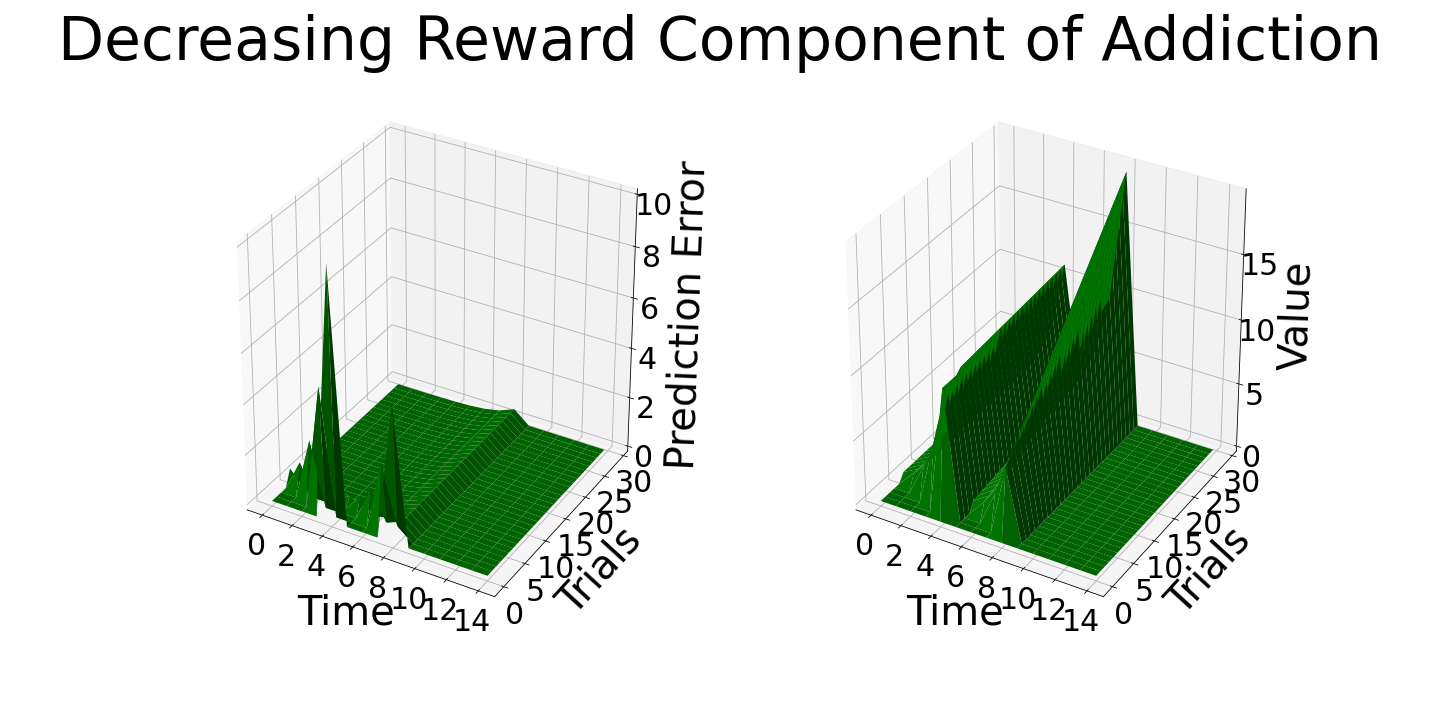
\includegraphics[width = 85mm]{graphs/cost_exp.png}
    \caption{Incrementally decreasing the value of the reward component of an addictive substance
    \newline \emph{An addicted agent was trained to expect a non-addictive reward (time = 4) and an addictive substance (time = 8). The addictive substance had a reward component valued at half that of the non-addictive reward. After learning to expect the addictive substance, subsequent trials decreased the value of the reward of the addictive substance. There is a drop in prediction error, but the value function still continues to increase.}}
    \label{fig:Baseline}
\end{figure}


\subsection{Experiment 3: Learning/Unlearning}
The goal of our final experiment is to examine the relationship between various TD-learning parameters and two potentially key components of the addiction discussion: time taken to learn addicted value structures, and time taken to "recover" from addiction (i.e. value structure returning to normal).

\subsubsection{Discount factor} We began by examining the effect of discount rate $\,\gamma\,$ on addiction and recovery. Note here that a higher discount factor leads to \textit{less} discounting of future values (with a discount factor of 1 valuing present and future values the same).

As the discount factor approached 1 (no discounting), the number of trials required to learn addicted values increased exponentially (Figure 9). This was likely due to the fact that our addictive substance occurred after the natural reward, meaning that an agent with less future discounting would include more of the addictive substance's value into account at the natural reward time-step. This finding is supported by our analysis of the effect of the discount factor on recovery rate, where we found that varying the discount factor had no effect on the number of trials required to unlearn the addicted values and return to a normal value table (i.e. recover from addiction) (Figure 10).

\begin{figure}[H]
   \centering
    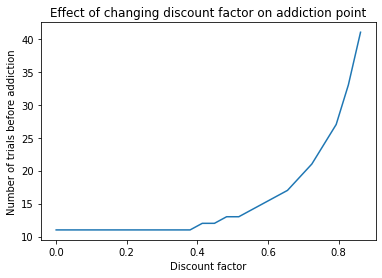
\includegraphics[width = 85mm]{graphs/discount_addiction.png}
    \caption{Increasing discount factor leads to slower addiction
    \newline \emph{Multiple models were trained with varying discount factors. The higher the discount factor, the longer the model took to become addicted.}}
    \label{fig:Baseline}
\end{figure}

\begin{figure}[H]
   \centering
    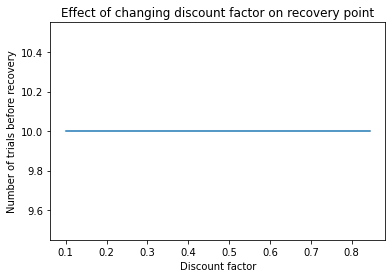
\includegraphics[width = 85mm]{graphs/discount_recovery.png}
    \caption{Increasing discount factor has no effect on recovery rate
    \newline \emph{Multiple models were trained with varying discount factors. There did not seem to be any relationship between discount factor and trials required to recover, likely due to the times at which the addictive substance and natural reward have been placed in the experiment.}}
    \label{fig:Baseline}
\end{figure}

\subsubsection{Learning factor}
The next parameter we examined was the learning factor $\eta$, which determines the importance of new information when revaluing a particular state (or, in our case, time-step). A higher learning factor means that more weight is placed on the most recent trial's rewards versus the previous trials' experience.

Higher learning factors lead to a significantly faster addiction point (Figure 11) because a larger portion of the extra addiction component is translated to future value. Due to the constant nature of this addiction component, a small increase in learning factor leads to a large decrease in addiction time.

\begin{figure}[H]
   \centering
    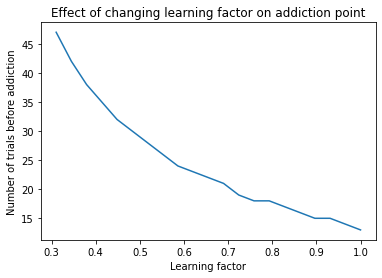
\includegraphics[width = 85mm]{graphs/learning_addiction.png}
    \caption{Increasing learning factor greatly reduces time to addiction
    \newline \emph{Multiple models were trained with varying learning factors. Increasing the learning factor (i.e. giving more weight to the most recent trial) greatly reduced the number of trials needed to learn an addicted value structure.}}
    \label{fig:Baseline}
\end{figure}

Both addiction point and recovery point behaved similarly in the face of varying learning factors (Figures 11 and 12), suggesting that RL agents that become more quickly addicted (i.e. have an earlier addiction point) can also recover quicker (i.e. have an earlier recovery point). Whether this extends to addiction in animals and humans is still to be verified.

\begin{figure}[H]
   \centering
    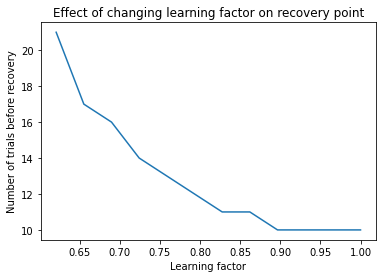
\includegraphics[width = 85mm]{graphs/learning_recovery.png}
    \caption{Increasing learning factor greatly reduces time to recovery
    \newline \emph{Multiple models were trained with varying learning factors. Increasing the learning factor (i.e. giving more weight to the most recent trial) greatly reduced the number of trials needed to unlearn an addicted value structure and return to baseline.}}
    \label{fig:Baseline}
\end{figure}



\subsubsection{Natural reward size}
We also examined how the size of the natural reward competing with the addictive substance affected the addiction and recovery points. As one would expect, a larger natural reward meant a later addiction point (Figure 13), as holding all else equal more trials were needed for an addictive substance to overcome a larger natural reward.

\begin{figure}[H]
   \centering
    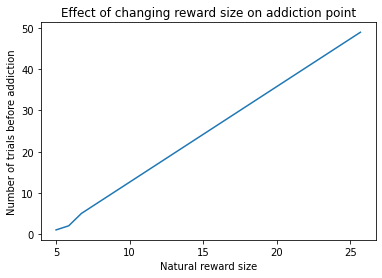
\includegraphics[width = 85mm]{graphs/reward_addiction.png}
    \caption{Increasing natural reward increases time to addiction
    \newline \emph{Multiple models were trained with varying natural reward sizes. The size of the natural reward scaled linearly with the addiction point, holding all else equal.}}
    \label{fig:Baseline}
\end{figure}

However, natural reward size appears to have no effect on recovery time (Figure 14). This is because the value table of an addicted agent does not undervalue a natural reward, but rather overvalues an addictive one. This means that no matter how large a natural alternative reward is, the time taken to recover remains the same.

\begin{figure}[H]
   \centering
    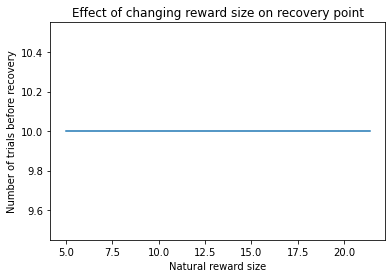
\includegraphics[width = 85mm]{graphs/reward_recovery.png}
    \caption{Increasing natural reward has no effect on recovery point
    \newline \emph{Multiple models were trained with varying natural reward sizes. The size of the natural reward had no effect on the recovery point.}}
    \label{fig:Baseline}
\end{figure}

\vspace{3em}

\subsubsection{Addictive substance size}
The last parameter we experimented on was the size (i.e. addiction component value) of the addictive substance. As expected, increasing the size of the addictive substance exponentially reduced the time before reaching addiction (i.e. earlier addiction point) (Figure 15). This is due to to the compounding effects of repeated trials and the fact that the addiction component is always a positive prediction error bump ($D_t > 0$).

\begin{figure}[H]
   \centering
    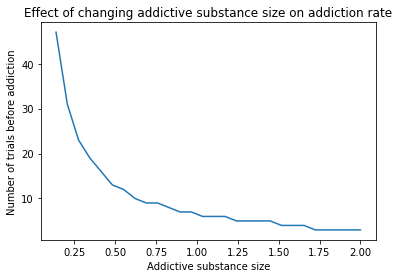
\includegraphics[width = 85mm]{graphs/substance_addiction.png}
    \caption{Increasing addictive substance size causes exponential reduction in addiction time
    \newline \emph{Multiple models were trained with varying addictive substance sizes. The size of the addictive substance drastically reduced the addiction point.}}
    \label{fig:Baseline}
\end{figure}

We found, however, that the size of the addictive substance did not have an effect on recovery time (Figure 16). This was due to the nature of our experiment and not necessarily a property of addiction in the RL model used. Since we removed the addiction component as soon as the agent became addicted, we did not allow the value table to become increasingly skewed (i.e. more addicted) through more trials. If we had left the addiction component for more trials, the time taken to recover would have increased and the size of the addictive substance would have factored in as well. However, we chose not to include these results as the time to recover would have been strongly tied to how long the addictive substance was left past the addiction point, which, although far from irrelevant, is a metric we did not experiment on.

\begin{figure}[H]
   \centering
    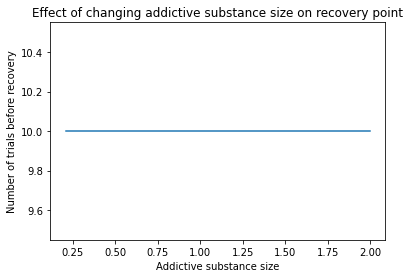
\includegraphics[width = 85mm]{graphs/substance_recovery.png}
    \caption{Increasing addictive substance size does not effect recovery time (in limited experiment)
    \newline \emph{Multiple models were trained with varying addictive substance sizes. The size of the addictive substance did not effect recovery time, under the specific condition that no time was given after initial addiction for the magnitude of addiction to increase.}}
    \label{fig:Baseline}
\end{figure}


\section{Discussion}
Human addiction is an extremely complex disorder, typically explained as having a strong relationship to dopamine. Addictive drugs have been shown to affect mechanisms of the brain that can be modeled using reinforcement learning algorithms, such as, for our case, temporal difference learning. Our goal was to use Reddish and Johnson's (2004) model of addiction as a basis for experimentation to further relate the results observed to human addiction.

This temporal difference reinforcement learning model was built on assumptions about cocaine \cite{ReddishJohnson2004}. Different classes of addictive drugs do not result in the same behavior with reference to human addiction, and thus this cannot be considered a model of all addictive substances, nor was that the goal in replicating this model. The focus was on how drugs like cocaine affect dopamine signaling (although, as previously discussed, many drugs have different effects on different systems, and dopamine is not the only mechanism involved in drug addiction).

The current model is based on the idea that addiction causes an agent to behave non-optimally as a result of a drug's effect on dopamine. The agent therefore learns "incorrectly" and values an addictive substance with a smaller reward more than a larger natural reward \cite{ReddishJohnson2004, ReddishJensenJohnson2008} (Appendix B: Figure 17). This was confirmed before starting any experiments (Figure 3), which shows that with all the same parameters, the value function associated with an addictive substance increases across trials, but the value function associated with a natural, non-addictive reward remains constant after training. This illustrates our definition of addiction which is consistent with the original model \cite{ReddishJohnson2004} as well as human addiction research which suggests that drugs are both rewarding and reinforcing after being repeatedly taken by someone susceptible to drug abuse \cite{Hyman2001, Koob1992}. After someone becomes addicted to a drug, it is common for periods of attempting to cease taking the drug to be followed by relapse and continued drug use \cite{Hyman2001}.

Our results suggest that even after removal of the reward component of an addictive substance the agent still values the substance higher than a natural reward (Figure 6). This is consistent with research on drug sensitization. Initially, the motivating factor for taking drugs is the positive rewarding "high" that results. The resulting pleasure often decreases over time and negative consequences begin to increase (i.e. health issues resulting from long-term drug use). Research has shown that continued drug use after its positive rewards decrease is typically associated with an attempt to re-experience the original positive rewards \cite{Hyman2001, Koob1992}.

Additionally, our results point to a potentially useful application of RL agents in the addiction space: mapping time taken to become addicted and recover from addiction to substances. Given the unethical nature of conducting such experiments on animals and/or humans, RL agents could provide a valuable proxy to help us better understand the relationships between various components of addiction (such as learning, discounting, reward and addiction size) and how easily one can become addicted, as well has how long it would take to recover from such addiction. The difficulty here would be tuning the various parameters of an RL agent to best fit real-world addiction scenarios and substances, but if that can be achieved to a sufficient degree of accuracy, the benefits could be significant.

\vspace{5.5em}

\section{Conclusion}
A successful temporal difference reinforcement learning model was replicated \cite{ReddishJohnson2004} based on the fact that cocaine causes a direct response in dopamine neurons. Prior to any experimentation we were able to confirm known patterns of the prediction error and the value function of the temporal difference learning algorithm in response to both natural, non-addictive, rewards as well as addictive substances. Through experimentation we were able to observe patterns seen in human addiction by comparing the outcomes of non-addictive agents and agents that were trained to expect addictive substances. It is important to note that the model used is not a comprehensive model of human addiction, but it does point out some important correlations to findings concerning human addiction from the literature as shown through the experiments performed as part of this project.


\section{Appendix A}
\begin{table}[H]
\begin{center} 
\caption{Baseline Parameters} 
\label{baselineparams} 
\vskip 0.12in
\begin{tabular}{ll} 
\hline
Parameter    &  Value \\
\hline
Reward       &   10 \\
Position~~~  &   7 \\
Max time~~   &   10 \\
Trials~~     &   10 \\
Eta~~~~~~~   &   1 \\
Gamma~~~     &   1 \\
\emph{Addiction}~  &   0.5 \\
\hline
\end{tabular} 
\end{center} 
\end{table}

\section{Appendix B}
\begin{figure}[H]
   \centering
    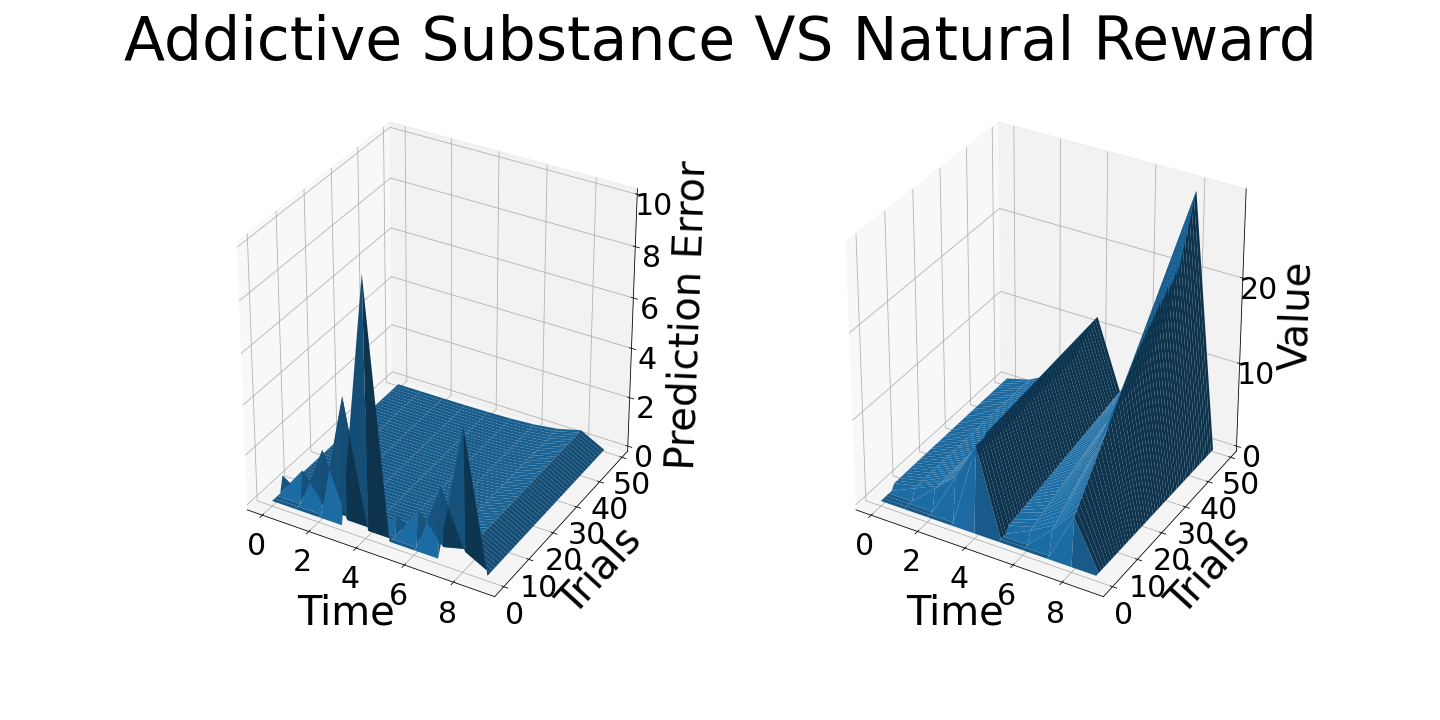
\includegraphics[width = 85mm]{graphs/both.png}
    \caption{Natural reward vs. addictive substance
    \newline \emph{A natural reward (time = 4) and an addictive substance (time = 8). The addictive substance is valued higher than the natural reward, even though the reward component of the addictive substance is half of the value of the natural reward.}}
    \label{fig:Baseline}
\end{figure}


\bibliographystyle{apacite}

\setlength{\bibleftmargin}{.125in}
\setlength{\bibindent}{-\bibleftmargin}

\bibliography{Galinho-Okun-Pant-ccm-final}

\end{document}
